% ==== Responsável: Rhayanne Borges ====
\chapter{Gerenciamento dos processos}\label{cap:processos}

\section{Programa e processo}\label{sec:programa-processo}
O conceito central em qualquer sistema operacional é o de processo. Um programa é um conjunto de instruções guardado em disco, sem consumir recursos. O processo é a instância desse programa em execução, que tem vida mais curta e precisa de memória, dispositivos de E/S e CPU. A \autoref{tab:prog-proc} resume a diferença.

\begin{table}[H]
  \centering
  \caption{Diferença entre programa e processo}\label{tab:prog-proc}
  \begin{tabularx}{\linewidth}{lXX}
    \toprule
    \textbf{Aspecto} & \textbf{Programa} & \textbf{Processo} \\
    \midrule
    Definição & Coleção de instruções que realiza uma tarefa & Instância de um programa em execução \\
    Duração & Mais longa & Mais curta \\
    Local & Armazenado no disco & Carregado na memória principal \\
    Recursos & Não requer recursos & Requer memória, E/S e CPU \\
    \bottomrule
  \end{tabularx}
  \legend{Fonte: adaptado dos slides de \citeonline{bourguet2026processos}.}
\end{table}

\section{Funções de um sistema operacional}

As funções do sistema operacional se dividem em cinco categorias de gerenciamento:

\begin{enumerate}
  \item \textbf{dispositivos de E/S}: aceita a entrada dos dispositivos de entrada e envia o resultado aos de saída, por meio dos \textit{device drivers};
  
  \item \textbf{arquivos}: cria e exclui diretórios e arquivos no sistema de arquivos da memória secundária;
  
  \item \textbf{processos}: gerencia a CPU, criando, agendando e encerrando os processos;
  
  \item \textbf{memória}: controla a alocação e a desalocação dos endereços de memória;
  
  \item \textbf{segurança}: protege o sistema, por exemplo com antivírus e \textit{firewall}.
  
\end{enumerate}

\section{\textit{Time sharing} e vida dos processos}

No \textit{time sharing}, a CPU alterna entre os processos executando cada um por milissegundos. Isso cria o \textbf{pseudoparalelismo}, a ilusão de paralelismo em uma máquina que, na prática, tem uma só CPU. Conceitualmente, cada processo possui sua própria CPU virtual, e o processo passa a maior parte da vida tentando acessar a CPU real.

O processador não sabe qual programa está em execução. Existe apenas um contador de programa físico, e a cada troca acontece o seguinte:
\begin{itemize}
  \item quando um processo é executado, o contador de programa lógico dele é carregado no físico;
  \item quando ele é interrompido, o contador físico é salvo no lógico.
\end{itemize}
Todas as informações do processo interrompido são salvas para que ele continue do ponto onde parou. A troca de um processo por outro é a \textbf{mudança de contexto}, e o conjunto de informações do processo é o seu \textbf{contexto}.

\section{Identificação de processos}

Cada processo é identificado por um número, o PID (\textit{Process Identifier}). Por meio do PID o sistema controla e interfere nos processos. O comando \texttt{pgrep} procura os processos pelo nome e devolve seus PIDs (\autoref{cod:pgrep}).

\begin{lstlisting}[language=bash, caption={Procurando o PID de um processo}, label={cod:pgrep}]
$ pgrep find
11122
\end{lstlisting}

\subsection{O diretório \texttt{/proc}}

O \texttt{/proc} é o sistema de arquivos do \textit{kernel} do GNU/Linux. Ele não contém arquivos reais, apenas informações do sistema, e por isso é um sistema de arquivos virtual. Cada diretório numerado corresponde ao PID de um processo em execução. Dentro de \texttt{/proc/<pid>} os principais arquivos são:

\begin{itemize}
  \item \texttt{cmdline}: argumentos da linha de comando do processo;
  \item \texttt{environ}: variáveis de ambiente visíveis ao processo;
  \item \texttt{fd}: descritores dos arquivos abertos;
  \item \texttt{exe}: link para o executável;
  \item \texttt{status}: estado do processo, uso de memória e outros dados;
  \item \texttt{task/<tid>}: informações das \textit{threads} do processo.
\end{itemize}

\begin{lstlisting}[language=bash, caption={Consultando um processo pelo \texorpdfstring{\texttt{/proc}}{/proc}}, label={cod:proc}]
ls /proc
cd /proc/$(pgrep firefox)
cat cmdline
cat status
cat oom_score
\end{lstlisting}

\section{Bloco de controle e tabela de processos}

O sistema mantém para cada processo um PCB (\textit{Process Control Block}) com todas as suas informações. Os PCBs ficam em uma área exclusiva da memória principal, cujo tamanho é definido pelo número máximo de processos suportados. A \textbf{tabela de processos} guarda um ponteiro para o PCB de cada processo, e o índice da entrada é o próprio PID, o que permite acessar o PCB rapidamente (\autoref{fig:pcb}).

\begin{figure}[H]
  \centering
  \caption{Tabela de processos e blocos de controle (PCB)}\label{fig:pcb}
  \begin{tikzpicture}[font=\small, every node/.style={align=center}]
    \matrix (t) [matrix of nodes, nodes={draw, minimum width=1.2cm, minimum height=0.6cm}, column sep=-\pgflinewidth, row sep=-\pgflinewidth] {
      |[fill=cyan!15]| PID & |[fill=cyan!15]| PCB \\
      1 & $\bullet$ \\
      2 & $\bullet$ \\
      $\vdots$ & $\vdots$ \\
      $n$ & $\bullet$ \\
    };
    \node[draw, rectangle split, rectangle split parts=6, fill=yellow!15, right=3.2cm of t, minimum width=3.4cm] (pcb)
      {Contador de programa \nodepart{two} Registradores \nodepart{three} Estado \nodepart{four} Prioridade \nodepart{five} Espaço de endereçamento \nodepart{six} Arquivos abertos};
    \node[above=0.1cm of pcb] {PCB};
    \draw[-{Stealth}] (t-2-2.center) -- ++(1.2,0) |- (pcb.west);
  \end{tikzpicture}
  \legend{Fonte: adaptado dos slides de \citeonline{bourguet2026processos}.}
\end{figure}

\section{Contexto de um processo}

O PCB guarda o contexto de hardware, o contexto de software e o espaço de endereçamento.

\subsection{Contexto de hardware}

O contexto de hardware armazena o conteúdo dos registradores e contadores da CPU. Esses valores são recarregados antes de o processo retomar a execução. Os principais são mostrados na \autoref{tab:registradores}.

\begin{table}[H]
  \centering
  \caption{Registradores que formam o contexto de hardware}\label{tab:registradores}
  \begin{tabularx}{\linewidth}{llX}
    \toprule
    \textbf{Sigla} & \textbf{Nome} & \textbf{Função} \\
    \midrule
    IR  & \textit{Instruction Register} & Instrução atual que está sendo executada \\
    PC  & \textit{Program Counter} & Endereço da próxima instrução a executar \\
    SP  & \textit{Stack Pointer} & Aponta para o topo da pilha do processo \\
    MAR & \textit{Memory Address Register} & Local dos dados para leitura ou gravação \\
    MBR & \textit{Memory Buffer Register} & Dados transferidos de e para a RAM \\
    AC  & Acumulador & Operações lógicas e aritméticas \\
    PSW & \textit{Program Status Word} & Estado da CPU e do programa em execução \\
    \bottomrule
  \end{tabularx}
  \legend{Fonte: adaptado dos slides de \citeonline{bourguet2026processos}.}
\end{table}

Os dados trafegam entre a CPU e a memória por quatro barramentos: de endereço, de dados, de instruções e de controle.

\subsection{Contexto de software}

O contexto de software reúne as características definidas na criação e na execução do processo:
\begin{itemize}
  \item \textbf{privilégios}: um processo com privilégios elevados acessa recursos críticos, enquanto um com privilégios baixos tem acesso restrito;
  \item \textbf{quotas}: limites de cada recurso que o processo pode alocar, com controle do limite e do uso atual;
  \item \textbf{informações de uso} (\textit{accounting}): tempo de CPU em modo usuário (\textit{user}) e em modo sistema, na execução de funções do \textit{kernel} ligadas ao processo.
\end{itemize}
São exemplos de quotas o número máximo de arquivos abertos, o tamanho máximo de memória principal e secundária alocada, o número máximo de operações de E/S pendentes e o tamanho máximo do \textit{buffer} de E/S\footnote{Disponível em: \url{https://linuxhint.com/set_max_user_processes_linux/}. Acesso em: 19 nov. 2026.}.

\subsection{Espaço de endereçamento}

É a área de memória do processo. Cada processo tem o seu, e o sistema o protege para que os outros processos não o acessem. Esse tema é detalhado na \autoref{cap:memoria}.

\section{Estados de um processo}

Durante a vida do processo, o acesso à CPU e aos recursos se altera, e isso acontece em função de eventos gerados pelo sistema ou pelo próprio processo. Um processo ativo está em um destes estados:

\begin{itemize}
  \item \textbf{execução} (\textit{running}): está usando a CPU;
  \item \textbf{pronto} (\textit{ready}): aguarda sua vez de ser executado;
  \item \textbf{espera} (\textit{waiting}): aguarda um evento ou recurso, como o fim da gravação de um arquivo ou uma determinada hora.
\end{itemize}

O sistema decide o escalonamento, isto é, a ordem e o critério com que os processos em estado pronto acessam a CPU. A \autoref{fig:estados} mostra as transições.

\begin{figure}[H]
  \centering
  \caption{Diagrama de estados de um processo}\label{fig:estados}
  \resizebox{\linewidth}{!}{\begin{tikzpicture}[font=\small, node distance=2.6cm, st/.style={draw, ellipse, minimum width=2cm, minimum height=0.9cm}, >=Stealth]
    \node[st] (cr) {criado};
    \node[st, right=of cr] (pr) {pronto};
    \node[st, right=2.8cm of pr] (ex) {execução};
    \node[st, right=2.2cm of ex] (te) {terminado};
    \node[st, below=2.2cm of $(pr)!0.5!(ex)$] (es) {espera};
    \draw[->] (cr) -- node[above]{admitido} (pr);
    \draw[->] (pr) -- node[above]{despacho} (ex);
    \draw[->] (ex) to[bend right=35] node[above]{interrupção} (pr);
    \draw[->] (ex) -- node[above]{fim} (te);
    \draw[->] (ex) to[bend left=15] node[right, xshift=2mm]{E/S ou evento} (es);
    \draw[->] (es) to[bend left=15] node[left, xshift=-2mm]{fim da E/S} (pr);
  \end{tikzpicture}}
  \legend{Fonte: adaptado dos slides de \citeonline{bourguet2026processos}.}
\end{figure}

\subsection{Criação e eliminação}

Na criação, o sistema adiciona um novo PCB e aloca o espaço de endereçamento na memória. A partir daí ele já reconhece o processo, que fica no estado \textit{criado} até ser admitido na lista de prontos. Na eliminação, os recursos são desalocados e o PCB é removido, mas o sistema ainda mantém na memória algumas informações do processo terminado.

\section{Média de carga}

A média de carga (\textit{load average}) é uma medida do \textit{kernel} do Linux que indica quantas solicitações de recursos do sistema estão pendentes. A cada cinco segundos o sistema conta os processos em espera e calcula uma média móvel exponencial para os últimos 1, 5 e 15 minutos. O comando \texttt{uptime} mostra os valores, e o \texttt{lscpu} informa o número de CPUs, pelo qual a média deve ser dividida.

\begin{lstlisting}[language=bash, caption={Média de carga com \texorpdfstring{\texttt{uptime}}{uptime} e \texorpdfstring{\texttt{lscpu}}{lscpu}}, label={cod:uptime}]
$ uptime
15:29:03 up 14 min, 2 users, load average: 2.92, 4.48, 5.20
$ lscpu | grep "^CPU(s):"
CPU(s):  4
\end{lstlisting}

Com 4 CPUs lógicas, a carga por CPU é $2{,}92/4 = 0{,}73$, $4{,}48/4 = 1{,}12$ e $5{,}20/4 = 1{,}30$ (\autoref{fig:load}). Valores abaixo de 1 indicam uso satisfatório dos recursos, acima de 1 indicam saturação, e uma fila de CPU inativa tem carga 0. Nesse exemplo a carga está diminuindo: no último minuto as CPUs ficaram em uso por cerca de 73\% do tempo, e nos 5 e 15 minutos anteriores o sistema esteve sobrecarregado em torno de 12\% e 30\%.

\begin{figure}[H]
  \centering
  \caption{Média de carga total e por CPU (exemplo do \texorpdfstring{\texttt{uptime}}{uptime})}\label{fig:load}
  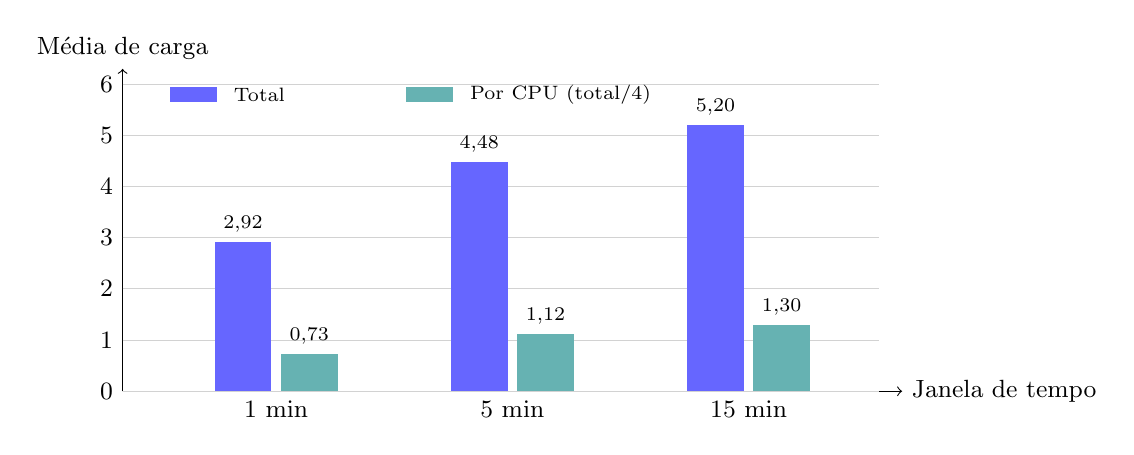
\begin{tikzpicture}[x=3.0cm, y=0.65cm, font=\small]
    
    \draw[->] (0.35,0) -- (3.65,0) node[right] {Janela de tempo};
    \draw[->] (0.35,0) -- (0.35,6.3) node[above] {Média de carga};

    \foreach \y in {0,1,2,3,4,5,6} {
      \draw[gray!35] (0.35,\y) -- (3.55,\y);
      \node[left] at (0.35,\y) {\y};
    }

    \fill[blue!60] (1-0.26,0) rectangle (1-0.02,2.92);
    \node[above, font=\scriptsize] at (1-0.14,2.92) {2,92};
    \fill[teal!60] (1+0.02,0) rectangle (1+0.26,0.73);
    \node[above, font=\scriptsize] at (1+0.14,0.73) {0,73};
    \node[below] at (1,0) {1 min};

    \fill[blue!60] (2-0.26,0) rectangle (2-0.02,4.48);
    \node[above, font=\scriptsize] at (2-0.14,4.48) {4,48};
    \fill[teal!60] (2+0.02,0) rectangle (2+0.26,1.12);
    \node[above, font=\scriptsize] at (2+0.14,1.12) {1,12};
    \node[below] at (2,0) {5 min};

    \fill[blue!60] (3-0.26,0) rectangle (3-0.02,5.20);
    \node[above, font=\scriptsize] at (3-0.14,5.20) {5,20};
    \fill[teal!60] (3+0.02,0) rectangle (3+0.26,1.30);
    \node[above, font=\scriptsize] at (3+0.14,1.30) {1,30};
    \node[below] at (3,0) {15 min};

    \fill[blue!60] (0.55,5.65) rectangle (0.75,5.95);
    \node[right, font=\scriptsize] at (0.78,5.8) {Total};

    \fill[teal!60] (1.55,5.65) rectangle (1.75,5.95);
    \node[right, font=\scriptsize] at (1.78,5.8) {Por CPU (total/4)};
  \end{tikzpicture}
  \legend{Fonte: os autores (2026), com os valores dos slides de \citeonline{bourguet2026processos}.}
\end{figure}